\documentclass[12pt,a4paper,twoside]{report}

\usepackage[utf8]{inputenc}
\usepackage{graphicx}
\graphicspath{ {./figures/} }
\usepackage{xcolor}
\usepackage{hyperref}
\usepackage{imakeidx} % for index
\makeindex[columns=3, title=Alphabetical Index]
\usepackage{soul} % allow wrapping of underlined text, via \ul{...}
\usepackage{natbib} % for bibliography
\usepackage[left=2cm,right=2cm]{geometry} % somewhat wider text to allow code
\usepackage{tikz} % add a few drawings ...
\usetikzlibrary{shapes.geometric, arrows} % for creating tikz flowcharts 
\tikzstyle{io} = [trapezium, trapezium left angle=70, trapezium right angle=110, minimum width=3cm, minimum height=1cm, text centered, draw=black, fill=blue!30]
\tikzstyle{process} = [rectangle, minimum width=3cm, minimum height=1cm, text centered, draw=black, fill=orange!30]
\tikzstyle{decision} = [diamond, minimum width=3cm, minimum height=1cm, text centered, draw=black, fill=green!30]
\tikzstyle{arrow} = [thick,->,>=stealth]

\usepackage{listings} % include source code files
% Solarized colour scheme for listings
\definecolor{solarized@base03}{HTML}{002B36}
\definecolor{solarized@base02}{HTML}{073642}
\definecolor{solarized@base01}{HTML}{586e75}
\definecolor{solarized@base00}{HTML}{657b83}
\definecolor{solarized@base0}{HTML}{839496}
\definecolor{solarized@base1}{HTML}{93a1a1}
\definecolor{solarized@base2}{HTML}{EEE8D5}
\definecolor{solarized@base3}{HTML}{FDF6E3}
\definecolor{solarized@yellow}{HTML}{B58900}
\definecolor{solarized@orange}{HTML}{CB4B16}
\definecolor{solarized@red}{HTML}{DC322F}
\definecolor{solarized@magenta}{HTML}{D33682}
\definecolor{solarized@violet}{HTML}{6C71C4}
\definecolor{solarized@blue}{HTML}{268BD2}
\definecolor{solarized@cyan}{HTML}{2AA198}
\definecolor{solarized@green}{HTML}{859900}

% Define C++ syntax highlighting colour scheme
\lstset{language=C++,
        basicstyle=\footnotesize\ttfamily,
        numbers=left,
        numberstyle=\tiny,
        tabsize=2,
        breaklines=true,
        escapeinside={@}{@},
        numberstyle=\tiny\color{solarized@base01},
        keywordstyle=\color{solarized@green},
        stringstyle=\color{solarized@cyan}\ttfamily,
        identifierstyle=\color{solarized@blue},
        commentstyle=\color{solarized@base01},
        emphstyle=\color{solarized@red},
        frame=single,
        rulecolor=\color{solarized@base2},
        rulesepcolor=\color{solarized@base2},
        showstringspaces=false
}

% include the external source file, instead of pasting its contents directly 
% into the LaTeX documen
\newcommand{\codelst}[1]{\lstinputlisting[caption=\texttt{\protect\detokenize{#1}}]{#1}\newpage}

% augment the paragraph skip ... a bit more clear text
\setlength{\parskip}{1em}

\bibliographystyle{plainnat}

\title{PhD Memo and Notes}
\author{Xanthos}
\date{\today}

\begin{document}

\begin{titlepage}
\maketitle
\end{titlepage}

%\frontmatter
\tableofcontents
\listoffigures
\listoftables

\chapter{Site Coordinates}
\label{ch:site-coordinates}

\emph{For the following we consider a site to mean a DORIS ground beacon.}

\section{tl;dr}
For consistency we are probably better off using DORIS site coordinates in the PDOP 
realization. Appropriate source code has been added to extrapolate site coordinates 
at a given epoch, using a corresponding DPOD SINEX file.

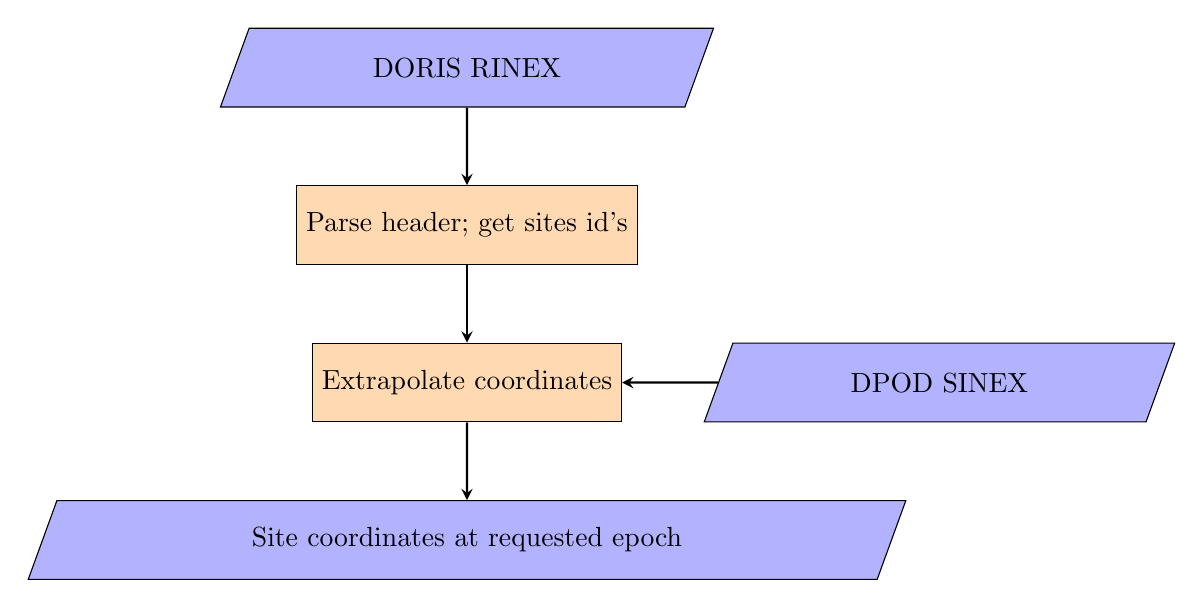
\begin{tikzpicture}[node distance=2cm]
\node (rnxin) [io] {DORIS RINEX};
\node (parsehdr) [process, below of=rnxin] {Parse header; get sites id's};
\node (xtrapolate) [process, below of=parsehdr] {Extrapolate coordinates};
\node (snxin) [io, right of=xtrapolate, xshift=4cm] {DPOD SINEX};
\node (out1) [io, below of=xtrapolate] {Site coordinates at requested epoch};
\draw [arrow] (rnxin) -- (parsehdr);
\draw [arrow] (parsehdr) -- (xtrapolate);
\draw [arrow] (snxin) -- (xtrapolate);
\draw [arrow] (xtrapolate) -- (out1);
\end{tikzpicture}

\section{DPOD}
For the analysis of DORIS observations, we need to have (at least approximate) 
site coordinates for the observed DORIS sites/beacons. Note that in DORIS RINEX 
v3 format \cite{DORISRNX3}, the RINEX files record all the observed sites at the 
file header, using the fields (among others):
\begin{itemize}
    \item 4-character station code,
    \item Station name (\textit{max 30characters long}) and 
    \item DOMES number
\end{itemize}

Example:
\begin{verbatim}
    51                                                      # OF STATIONS
D01  AMVB AMSTERDAM                     91401S005  3   0    STATION REFERENCE
D02  MAUB MARION ISLAND                 30313S005  3   0    STATION REFERENCE
...
D50  BADB BADARY                        12338S002  3   0    STATION REFERENCE 
D51  GRFB GREENBELT                     40451S178  3   0    STATION REFERENCE
\end{verbatim}

To match the sites with external sources (e.g. SINEX files), we will normally use 
the 4-character station code and/or the domes number.

In the meeting on the 15\textsuperscript{th} October 2021, it was suggested that instead of ITRF(2014, ...) 
we should better use the IDS published DPOD set of coordinates/veclocities (for better 
consistency). PDOP is a ``DORIS extension of the ITRF for Precise Orbit Determination'' 
estimated and delivered by the IDS Combination Center; details can be found on the 
\href{https://ids-doris.org/analysis-coordination/combination/dpod.html}{IDS DPOD webpage}.

Currently (October 2021) the latest PDOP realization is DPOD2014 \cite{Moreaux2019118} and 
the latest release is ``August 2020 - version \#5 - \textbf{dpod2014\_0}'' \cite{Moreaux2020};
the corresponding information files are published by 
\href{ftp://cddis.gsfc.nasa.gov/pub/doris/products/dpod/dpod2014/}{cddis} and
\href{ftp://doris.ensg.ign.fr/pub/doris/products/dpod/dpod2014/}{ign} in both 
SINEX and ascii/text format. Of the two, we are going to use the SINEX files (since 
they are more comprehensive, self-contained, capable of holding much more detailed information 
and widely used is Satellite Geodesy). 

Appropriate source code is written so as to be able to read and parse the DPOD SINEX 
file(s) and extrapolate site coordinates to a desired epoch. The sites we want to 
extrapolate coordinates for, are distinguished via their 4character id.

\section{Todo}
\subsection{Coordinate Std Deviations}
Also compute (extrapolated) coordinate stdandard deviations to go with the computed coordinate components.

\subsection{Ignored SINEX Sections}
The \textbf{dpod2014\_0} SINEX file contains a couple of blocks that (at this point) are 
not considered when parsing/extrapolating. These are (\cite{Moreaux2020}):
\begin{itemize}
    \item SOLUTION/DISCONTINUITY: origin (ex: earthquake, beacon change, antenna problem...) of
the position discontinuities
    \item SOLUTION/DATA\_REJECT: periods of time not included in the combination
    \item STATION/TO\_BE\_UPDATED: stations with non-negligible position change wrt DPOD2014v03
\end{itemize}

These are not crucial at this point but should be considered further on.

\section{Technicalities}

Main source code for the above is developed within the 
\begin{itemize}
    \item \href{https://github.com/xanthospap/libsinex}{sinex} and
    \item \href{https://github.com/xanthospap/doris}{doris}
\end{itemize}
repositories.

%The main function that does the work, is:
%\begin{lstlisting}
%#if __cplusplus >= 202002L
%template <typename T>
%    requires(T::is_of_sec_type && !std::is_same_v<T, dso::microseconds>)
%#else
%template <class T,
%          typename = std::enable_if_t<(T::is_of_sec_type) &&
%                                      (!std::is_same_v<T, dso::microseconds>)>>
%#endif
%int extrapolate_sinex_coordinates(
%            const char *snx_fn, char **site_ids, int num_sites,
%            const dso::datetime<T> &t) noexcept {
%    dso::datetime<dso::microseconds> t_micro =
%    t.template cast_to<dso::microseconds>();
%return extrapolate_sinex_coordinates(snx_fn, site_ids, num_sites, t_micro);
%}
%\end{lstlisting}

The following example (\href{https://github.com/xanthospap/doris/blob/main/test/test\_pdop\_crd.cc}{test\_pdop\_crd.cc}) 
extrapolates the coordinates of all the sites recorded in a DORIS RINEX file using a DPOD 
SINEX file. It is tested with the following SINEX files:
\begin{itemize}
    \item dpod2014\_053.snx
\end{itemize}

%\codelst{source/test_pdop_crd.cc}

\bibliography{doris}

\printindex

\end{document}